\section{Materials and Methods}
% The materials and method section should describe in detail the procedures followed, indicating an awareness of any likely pitfalls or problems with the techniques. Published techniques need not be described in detail but should be referenced. The student should demonstrate an understanding of established techniques. \underline{N.B.} no results obtained by the student should appear in this section.
% 
% \begin{itemize}
 % \item Does this section describe in detail the procedures followed? Could you carry out this project following the methods reported here?
% \end{itemize}

% \begin{figure}[h]
	% \begin{center}
    % \includegraphics{es3d.pdf}
	% \end{center}
    % \caption{Example of an embedded pdf}
% \end{figure}

\subsection{Data Sources}
% WHERE THE DATA COME FROM
% WHAT THOSE DATA ARE
% FIGURE OF DATA SOURCES -> MYSQL DB WITH NAME OF SCRIPTS
% FIGURE OF DATABASE SCHEMA

The DomVizApp database was built by importing and linking the following sources: Pfam \cite{pfamdb}, Uniprot \cite{uniprot}, PDB \cite{pdb} and Drugbank \cite{drugbank}.

A collection of Perl modules were written to perform data pre-processing and to import the data into a MySQL\footnote{http://www.mysql.com/} database which acts as the master data store. These Perl scripts allow databases to be created given new data from Pfam, Uniprot or the PDB. Importing the data into a general purpose database allows us to easily integrate our data sources, facilitates flexible querying for analysis and allows for additional annotation in the future. The data sources, import scripts and database schema are illustrated in Figure~\ref{dataimport} and described below.  

\begin{figure}[h]
 \begin{center}
 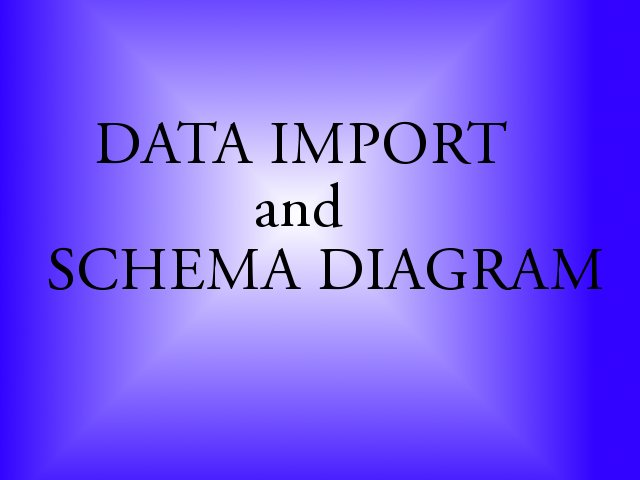
\includegraphics[scale=0.5]{figures/placeholder_dataimport.jpg}
 \end{center}
 \caption{Overview of data sources and target schema}
 \label{dataimport}
\end{figure}

\subsubsection{Pfam}
Domains and architectures form the foundation of DomVizApp and were imported from Pfam version 22.0, available from the Pfam FTP site\footnote{ftp://ftp.sanger.ac.uk/pub/databases/Pfam/current\_release/swisspfam.gz}. The swisspfam dataset contains all the domains belonging to a sequence. Domains aren't presented linearly and the file requires additional parsing in order to extract the sequence's architecture. We extracted and loaded the sequence accession, Swissprot name and stored the sequence's architecture as a string with a dot-separated format (e.g. \texttt{D1.D2.D3.D1.D1}). The list of all Pfam clans (Pfam-C.gz) was also imported so that those domains that belonged to clans could be associated with other sibling domains. 

The dataset contains 45,684 distinct architectures (ignoring Pfam-B domains) from 9,318 domains, *fillme* of which are members of one of *fillme* clans.

\subsubsection{Uniprot}
In order to link domain architectures to sequences and taxonomy, Uniprot v14.0 (Swissprot 56.0) protein data were imported. The data includes all accession numbers for Swissprot entries, which allows us to link drug targets with Pfam sequence entries. We are also able to group sequences by identical domain organizations. This release contains 392,667 UniprotKB/Swissprot entries. % todo: only swissprot entries?

\subsubsection{PDB}
The PDB records were used to determine protein sequences that have had their structure solved. DomVizApp uses this information to allow users to filter for architectures that belong to a sequence that has had its structure determined. Links between PDB chain and Uniprot are only available in separate downloads for each individual chain from the Worldwide Protein Data Bank (wwPDB). Rather than downloading and parsing the full PDB database, we used the PDBSprotEC mappings \cite{pdbsprotec} which are available from the Bioinformatics Group at UCL\footnote{http://www.bioinf.org.uk/pdbsws/}. The dataset has 110,858 PDB chains mapped to *fillme* distinct Swissprot sequences. 

\subsubsection{DrugBank}
To analyse the targetting of proteins by drugs, details of drugs and their corresponding targets were obtained from the DrugBank \cite{drugbank} drugset as of 14 June 2008. The full drugcard set contains comprehensive drug data combined with drug-target data, such as sequence, Swissprot identifier and GO classification information. It also includes Pfam domains for each of the targets but it simply lists all the domains belonging to the target, not specifically the domains targetted by the drug. Only approved drug targets were considered in the analysis. The full drugcard set lists 4,764 drugs of which 1,484 are flagged as `Approved'. For our analysis, we only considered human targets.

\subsection{Domain Architecture Analysis}
% DESCRIBE ANALYSIS PERFORMED
% HOW THEY WERE PERFORMED
% WHY THEY WERE PERFORMED
After loading and integrating the different data sources, and having performed the necessary normalization of Pfam and Drugbank sequence accession numbers to the Uniprot primary accession number, we were able to perform some general analysis of the protein domain and architecture landscape. Using progressively selective criteria, we were able to retrieve summary information related to protein sequence Pfam entries, human protein domains and commonly occuring architectures.

For the first stage of analysis, a collection of SQL scripts were written to summarize the number of distinct domains and architectures and how frequently these domains and architectures occurred in sequences. We extracted this information for all species and HomoSapiens.

We also analysed the occurrences of domains in architectures, which required development of MySQL stored procedures as the information could not be retrieved using standard SQL set operations. We obtained these totals by getting a list of distinct domains and then iteratively searching for architectures that contained these domains. We retrieved total and HomoSapien numbers.

As mentioned previously, the purpose of this analysis was to survey the domain architecture landscape. As DomVisApp draws network graphs of related architectures, we wanted to have a sense of how large a typical graph would be (i.e. number of nodes) and what might be the worst case scenario. We were also able to see what types of domains were frequently occuring and investigate what was their related function.

The second stage of analysis was to investigate the possible number of `druggable' proteins in the human genome. Using the current DrugBank drug-target data we summarized the number of approved drugs currently targetting human proteins. We then retrieved additional protein sequences that had the same architecture as drug-targets but weren't currently targetted by any drugs.

To improve the number of probable druggable proteins, we should also include those sequences which have some of the domains (or all domains but in a different architecture) that specifically bind the drug. However, Drugbank does not currently state explicitly which domain the drug targets. We calculated the number of sequences that contain one or more of the same domains as the drug-target protein. This is likely to return an inflated figure as it is unlikely that a drug targets all the domains in a target protein.

This shortcoming is a reason that one of the goals of DomVizApp is to assist bioinformaticians to interactively explore protein architectures by allowing them to indicate domains of interest (say, a domain known to bind a drug) and then update the network graph accordingly.

\subsection{DomVizApp Implementation}
% EVERYTHING THAT THE APPLICATION DOES AND USES

Given a protein chain, the application first retrieves the architecture of the chain (the `parent architecture'). It then finds all architectures that share one or more domains with the parent architecture.  These architectures, and chains with these architectures, are then visualised as a network graph.

The visualisation application was implemented in Java. Core libaries that were used include the Lucene engine (http://lucene.apache.org/) which was used to create high-performance search indexes. All protein domain and associated data was stored as a Lucene document. The Prefuse library (http://prefuse.org/) was used to model and visualize the network graph.

\subsubsection{Lucene Indexing Engine}
% Details of what the Lucene engine does for you and how exactly you used it for indexing your data
A searchable Lucene index was then created from the collected MySQL data. A small Java program was written to generate the search index. 

\subsubsection{Prefuse Graph Library}
% Same as Lucene. A figure helps.
There are several algorithms available for constructing network drawings. The Prefuse library provides many layout algorithms which can be customised based on requirements. The application uses a force-directed layout \cite{force} which attempts to place all the nodes by modelling edges as springs. These bring connected nodes together and spread unconnected nodes apart until the forces reach equilibrium, resulting in relatively attractive drawings. As this layout algorithm can be CPU-intensive, we allow the user to stop the the algorithm when a reasonable layout has been acheived.
\subsubsection{Force-Directed Layout}
The spring force of an edge which joins architecture nodes is manipulated based on the similarity score of the architectures. This modification brings architectures that are more similar than others closer together in the layout. 
\subsubsection{User Interface}
s

\subsection{Computing the scores for architecture similarity}

In order for the application to render a network graph, architectures are represented as nodes and are joined to other architectures with an edge based on architecture similarity.

In this application, we apply a well-known alignment technique to compare architectures and use the resulting score to create relationships between similar architectures. First, given two architectures, a similarity matrix is created to score the similarity between each pair of domains. 

In the similarity matrix, the score assigned to each pair of domains may be simple, indicating a straighforward match or mismatch, or it may be related to one of the above mentioned techniques for relating domains.

During development, we initially used a simple match/mismatch scoring. The varying heuristics and scoring techniques available result in different relationships among sets of architectures and hence different graphs.

In the current implementation of the application, we use a scoring matrix that measures domain similarity based on:
\begin{enumerate}
	\item Domains matching exactly
	\item Domains belonging to the same clan
	\item Domain mismatch
\end{enumerate}

Given the generated similarity matrix we then use the Needleman-Wunsch algorithm \cite{nwalgo} to perform an alignment of the sequence of domains in two architectures and obtain a maximal alignment score.

Using this technique on a given set of architectures, scores are calculated for every possible pair of architectures.

% FIGURE showing example of scoring

\subsection{Using Matrix of Scores to Draw Network Graph}

To visualize a set of architectures as a network graph, the calculated maximal scores are used to pair-up each architecture in the set and create an edge between the two architecture nodes. The procedure is as follows:

$C$ is the set of connected architectures, initialised with only the parent architecture. $U$ is the set of unconnected architectures, initialised to all other architectures of interest. $S$ is the matrix of scores, where $S_{i,j}$ is the maximal calculated alignment score for architectures $i$ and $j$. Finally, to create edges between architecture nodes:
\begin{algorithmic}
\WHILE{$U \neq \emptyset$}
\STATE Get maximum $S_{i,j}$ where $i \in C$ and $j \in U$.
\STATE Create edge between architectures $i$ and $j$.
\STATE Remove $j$ from $U$ and add to $C$.
\ENDWHILE
\end{algorithmic}
In this manner, each architecture in the set of unconnected architectures is removed and connected to another which has the maximal similarity score.

If there are two or more architecture pairs with the same similarity score, the chosen relationship is random unless one of the pairs include the parent architecture of interest. In this case, the pair which includes the parent architecture is preferred. Therefore, the resulting graph may not be the only graph that represents the pairing of architectures with maximum scores. 

\subsection{Graph layout \& filtering}
Architectures and, optionally, chains are represented as nodes on the graph. All chains are connected to their architecture. Architectures are connected by an edge to other architectures based on the results of the joining algorithm described above.  





